\documentclass[pscyr,nonums]{hedlabwork}
\usepackage[russian]{babel}
\usepackage[utf8]{inputenc}
\usepackage{hedmaths}
\usepackage{graphicx}

\labnum{666}
\labname{Исследование физических свойств сатанистов}
\student{Иванов И. И.}

\begin{document}
  \makeheader

  \emph{Цель работы:} изучение спектра поглощения и упругости костной ткани
    сатанистов.

  \emph{Используемые при расчетах формулы и значения:}
  \( S = 2,\!3\cdot10^{-5}~\text{м}^2; \ \sigma = \dfrac{JU}{S(T^4 - T_0^4)} \).

  \begin{figure}[h!]
    \center
    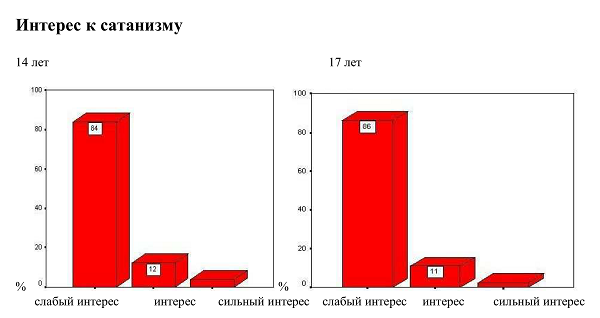
\includegraphics[width=.6\textwidth]{image} \\
    \caption{Результаты опросов среди несовершеннолетних}
  \end{figure}

  \emph{Вывод:} придумайте сами. Дети любознательны, естественно им это
    интересно.
\end{document}
